\section{Motivation}
\begin{figure}[!t]
\centering
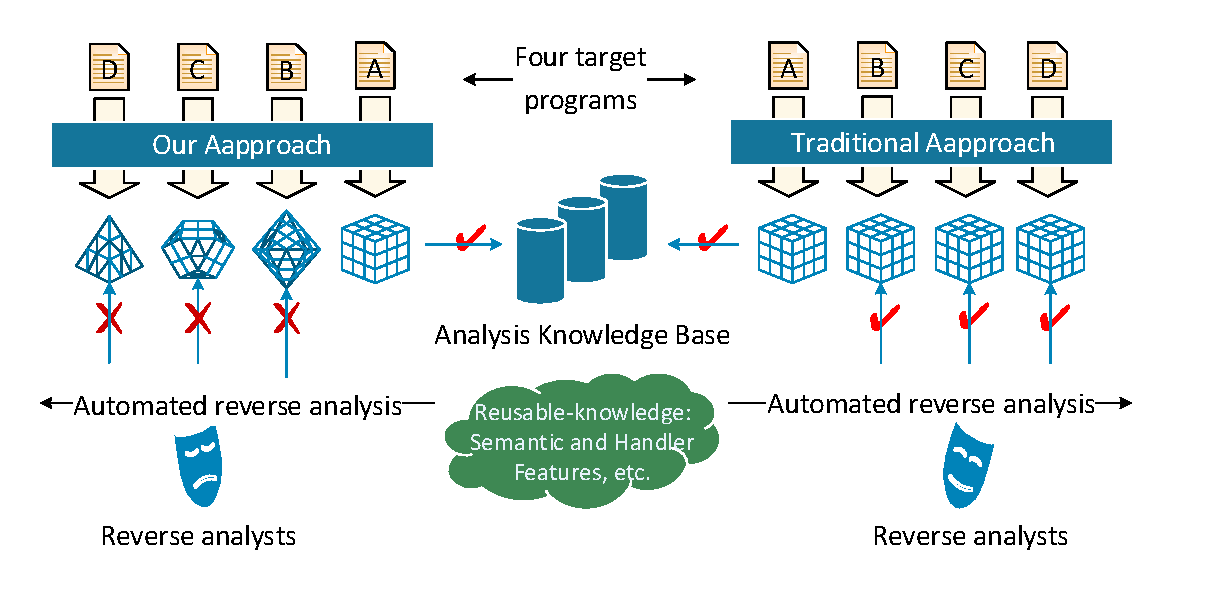
\includegraphics[width=0.75\columnwidth]{fig/figone.pdf}
\caption{The process of reusing attacking knowledge for code reverse engineering.
Here we have four different target programs, A, B, C and D.
In the right side of the scenario, all programs are obfuscated with a code obfuscation scheme that a virtual instruction will be deterministically translated to a fixed set of native code.
This allows an attacker to reuse knowledge obtained from one program to efficiently reverse engineer other programs.
In another scenario, the mapping between virtual instructions and native code is different for different programs.
In this way, the attacker is  unable to reuse the previously extracted knowledge to perform reverse analysis across programs.}
\label{fig:one}
\end{figure}

Figure~\ref{fig:one} depicts an reverse analysis scenario where an analyst can
reuse the \textit{analysis knowledge} to attack applications protected by
the same VM-based code obfuscation scheme. In this example, there are four different programs
to be protected, labelled as A, B, C and D. In the right side of the diagram,
all the four programs are protected using an identical set of virtual
instructions and bytecode handlers. Under this setting, an experienced analyst would be able to
use the knowledge of the mapping of virtual instructions and bytecode handlers obtained
from one program to reverse-engineer the other three programs. Bear in mind that,
uncovering the mapping between virtual instructions and native code is often the most
time-consuming process for attacking VM-based code obfuscation. Having able to
reuse the attacking knowledge thus can significantly reduce the cost involved in the
attack.
In another scenario, the translations between virtual instructions and native code
vary among programs. Therefore,  the
knowledge obtained from one program will be in inapplicable to others.
This forces the analyst to start from the scratch when reverse engineering a new program.
This  example shows that shuffle the relationship between the virtual instructions and bytecode handlers
can significantly increase the effort and cost involved in performing the attack.
In the remainder section, we describe how we can construct such as scheme in details.  